\section{Installazione}
Il deploy e la configurazione dell'intero sistema consistono di un numero considerevole di procedure non banali da applicare.\\
In accordo con il proponente \PROPONENTE, il quale è anche l'utilizzatore del prodotto, verranno fornite da quest'ultimo le credenziali di accesso ai servizi esterni e piattaforme elencate in \ref{configurazione}, in maniera tale che le attività di deploy e configurazione siano realizzate dal team \GRUPPO.\\
Tuttavia, viene di seguito esposto come fare il deploy e la configurazione del sistema.
\subsection{Download}\label{download}
Per scaricare l'applicativo è sufficiente clonare o scaricare il repository disponibile al link \url{https://github.com/CoCodeSWE/AtAVi} (2017-05-02).

\subsection{Configurazione}\label{configurazione}
Per il \gl{deploy} dei servizi del prodotto, è necessario prima di tutto creare e configurare alcuni account per il corretto funzionamento del prodotto.

\subsubsection{Amazon Web Services}
\paragraph{Creazione}
Amazon Web Services è una collezione di servizi di cloud computing che compongono la piattaforma "on demand" offerta dall'azienda Amazon. Questi servizi sono operativi in 12 regioni geografiche in cui Amazon stessa ha suddiviso il globo.\\
I servizi utilizzati dal prodotto sono:
\begin{itemize}
	\item API Gateway;
	\item Simple Notification Service;
	\item Lambda;
	\item DynamoDB.
\end{itemize}
Per usufruire di essi, è sufficiente creare un account alla pagina \url{https://aws.amazon.com} (visitato in data 2017-05-02) cliccando sul pulsante "Registrazione". \\
Durante la registrazione, verrà chiesto di associare una carta di credito all'account. Questa operazione deve essere fatta, altrimenti non sarebbe possibile fare utilizzo dei servizi offerti.
\begin{figure}[h]
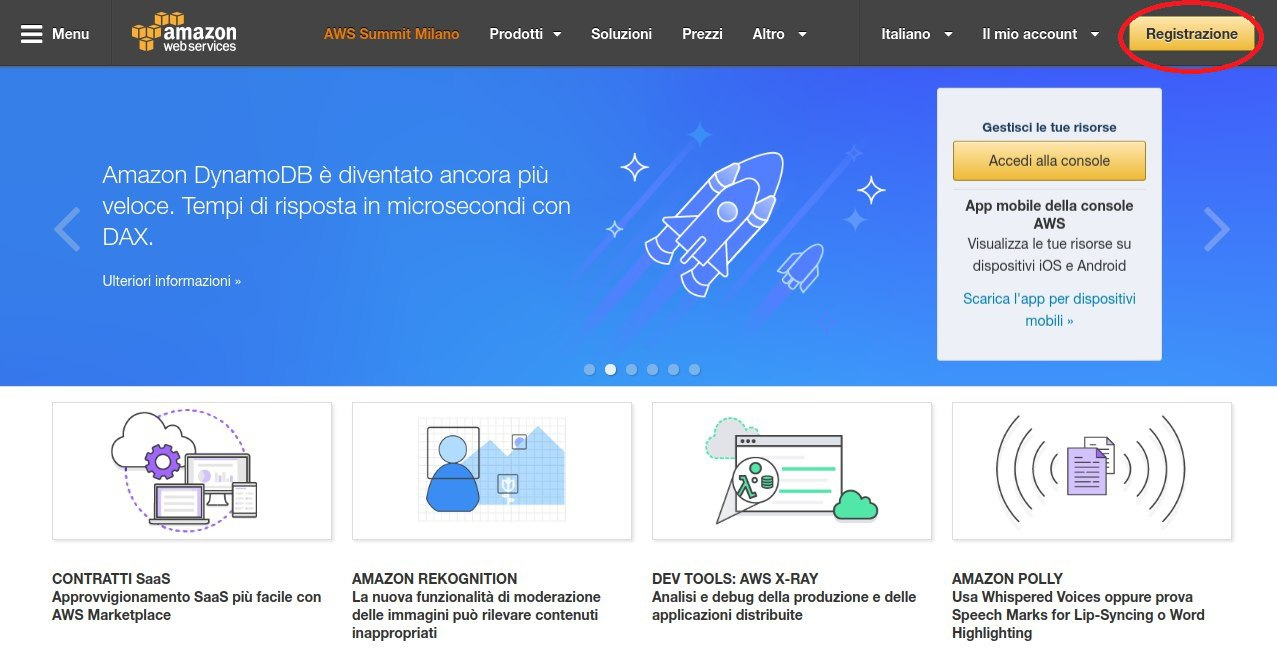
\includegraphics[width=\textwidth,height=\textheight,keepaspectratio]{sezioni/images/aws.jpg}
\caption{Registrazione AWS}
\end{figure}

\subsubsection{Serverless}
\paragraph{Creazione}
Serverless è un framework per alcuni servizi di cloud computing, tra i quali quelli di Amazon Web Services. È un progetto molto giovane, ma che gode già di un ottimo supporto.\\
Esso permette la realizzazione e il deploy dei servizi in maniera molto più facile e veloce, infatti l'effettivo deploy del sistema è semplificato, velocizzato e automatizzato grazie ad esso. \\
È necessario installare il framework lanciando il comando \file{npm install serverless -g} nel terminale.
\paragraph{Configurazione}
Una volta installato, è necessario applicare la seguente procedura:
\begin{itemize}
	\item creare delle AWS Access Key seguendo le istruzioni presenti al link \url{https://serverless.com/framework/docs/providers/aws/guide/credentials#creating-aws-access-keys} (visitato in data 2017-05-02);
	\item fornire le credenziali create seguendo le istruzioni al link \url{https://serverless.com/framework/docs/providers/aws/guide/credentials#setup-with-serverless-config-credentials-command} (visitato in data 2017-05-02);
\end{itemize}

\subsubsection{Microsoft Speaker Recognition}\label{speakerRec}
\paragraph{Creazione}
Questo servizio viene utilizzato per realizzare le funzionalità che richiedono il riconoscimento vocale, quali la costruzione dell'impronta vocale (\gl{enrollment}) di un nuovo amministratore e l'accesso al sistema.\\
È necessario creare un account al link \url{https://www.microsoft.com/cognitive-services} (visitato in data 2017-05-02) cliccando sul pulsante "Get started for free".
\begin{figure}[h]
	\centering{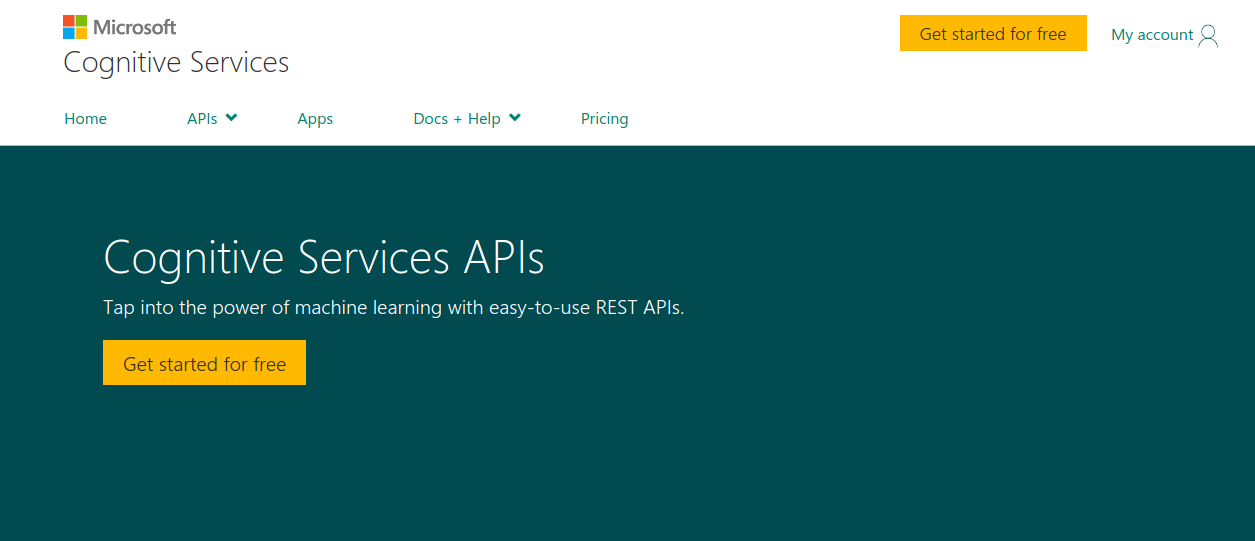
\includegraphics[width=0.8\textwidth,height=\textheight,keepaspectratio]{sezioni/images/microsoft.png}}
	\caption{Registrazione Microsoft Cognitive Services}
\end{figure}
\paragraph{Configurazione}

\subsubsection{IBM Watson Speech to Text}
\paragraph{Creazione}
Questo servizio viene utilizzato per realizzare le funzionalità di Speech to Text, ovvero l'estrazione del testo pronunciato in un file audio.\\
È necessario creare un account su IBM Bluemix al seguente link \url{https://console.ng.bluemix.net/registration/?target=/catalog/\%3fcategory=watson} (visitato in data 2017-05-02). Vengono concessi 30 giorni di utilizzo gratuito, oltre i quali è necessario associare una carta di credito all'account.
\begin{figure}[h]
	\centering{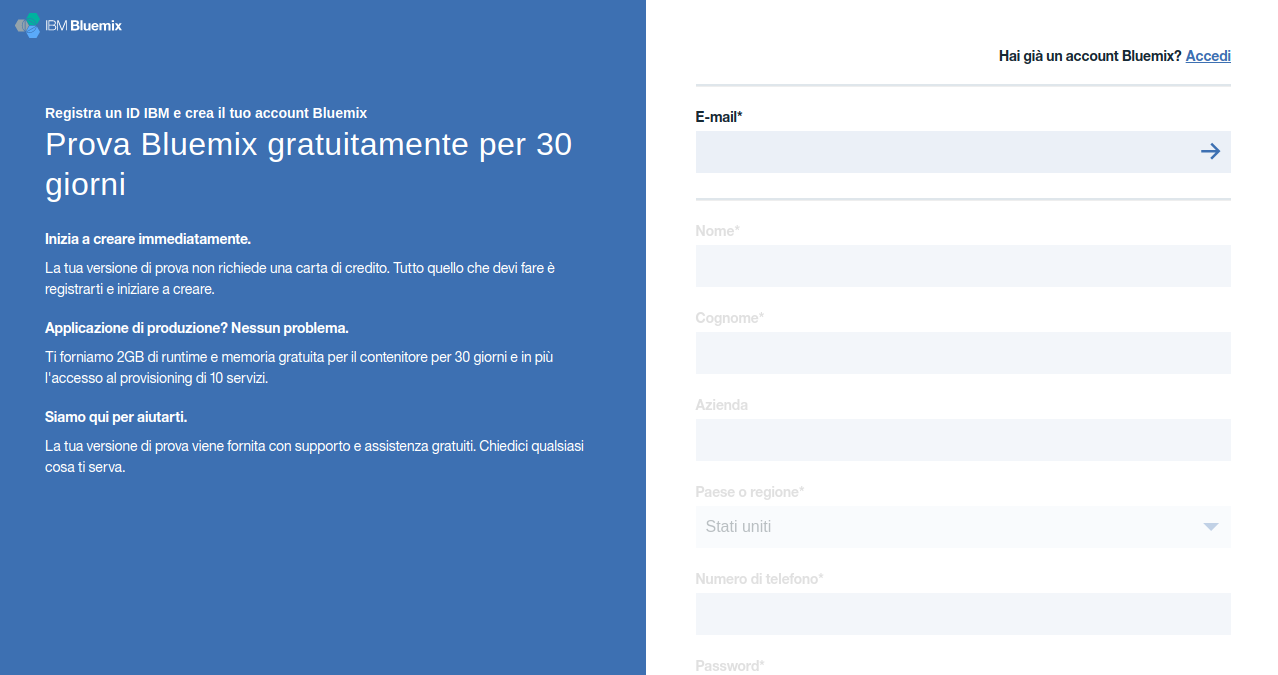
\includegraphics[width=0.8\textwidth,height=\textheight,keepaspectratio]{sezioni/images/bluemix.png}}
	\caption{Registrazione bluemix}
\end{figure}
\paragraph{Configurazione}
Una volta effettuato l'accesso, è necessario applicare la seguente procedura:
\begin{itemize}
	\item accedere alla sezione dei servizi Watson \url{https://console.ng.bluemix.net/catalog/?category=watson} (visitato in data 2017-05-02) e cliccare sul servizio di Speech to Text (figura);
	\item copiare le credenziali di utilizzo (username e password) e attivare il servizio (figura);
	\item SETTARE LE CREDENZIALI NEL SOFTWARE
\end{itemize}
\subsubsection{api.ai}
\paragraph{Creazione}
È il Software Development Kit (SDK) utilizzato per l'effettiva costruzione dell'assistente virtuale.
È necessario creare un account al link \url{https://api.ai/} (visitato in data 2017-05-02) cliccando sul pulsante "sign up free", ma se si dispone già di un account Google, Facebook, Slack o Github è possibile effettuare l'accesso tramite uno di essi cliccando sul pulsante "log in".
\begin{figure}[h]
\centering{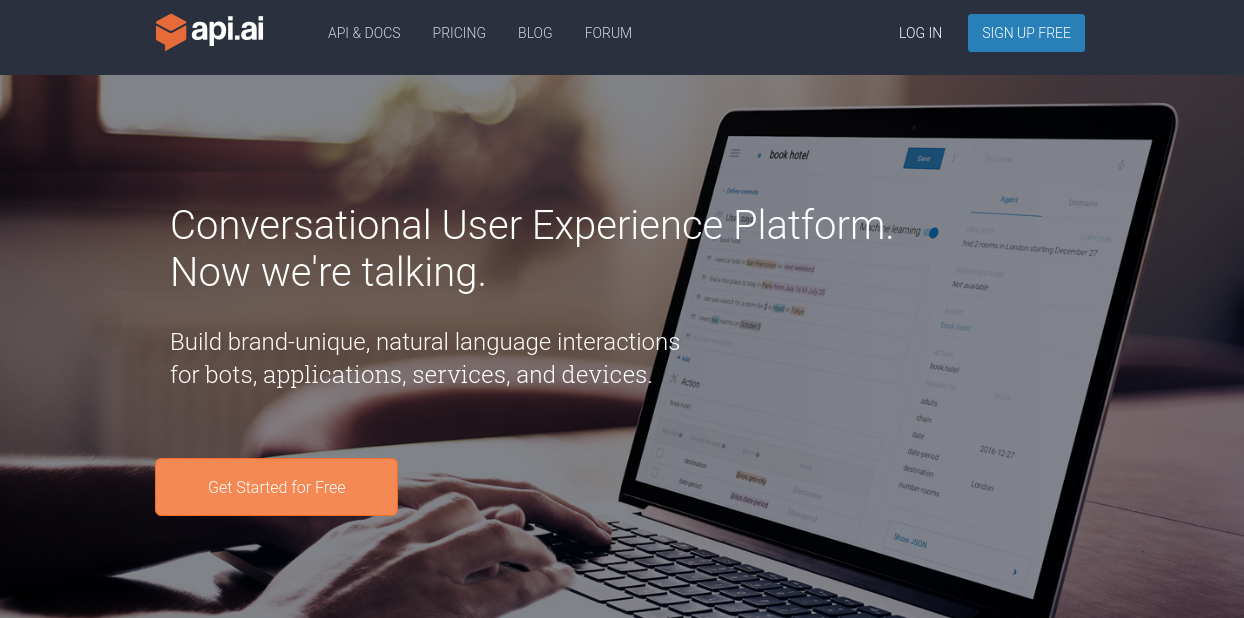
\includegraphics[width=0.7\textwidth,height=\textheight,keepaspectratio]{sezioni/images/apiai.png}}
	\caption{Registrazione api.ai}
\end{figure}
\paragraph{Configurazione}
Dopo aver effettuato l'accesso, selezionare il menù degli \gl{agent} a sinistra (figura \ref{fig:menuapi}) e scorrerlo fino in fondo, selezionando "Create new agent" (figura \ref{fig:newAgent}). \\
\begin{figure}[h]
	\centering{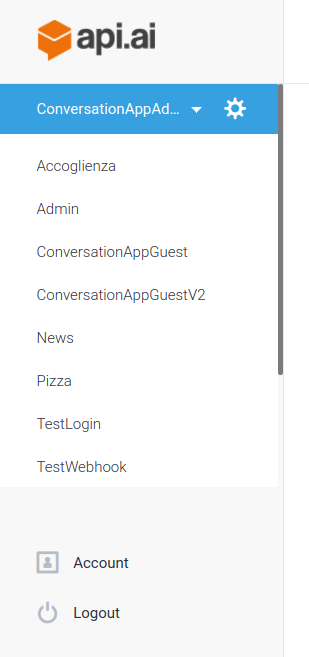
\includegraphics[width=0.3\textwidth,height=\textheight,keepaspectratio]{sezioni/images/menuapi.png}}
	\caption{menu agent api.ai}\label{fig:menuapi}
\end{figure}
\begin{figure}[h]
	\centering{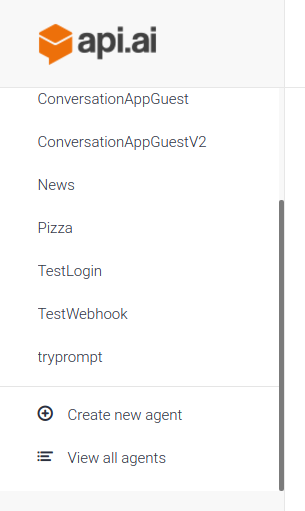
\includegraphics[width=0.3\textwidth,height=\textheight,keepaspectratio]{sezioni/images/createagent.png}}
	\caption{nuovo agent api.ai}\label{fig:newAgent}
\end{figure}

\begin{figure}[h]
	\centering{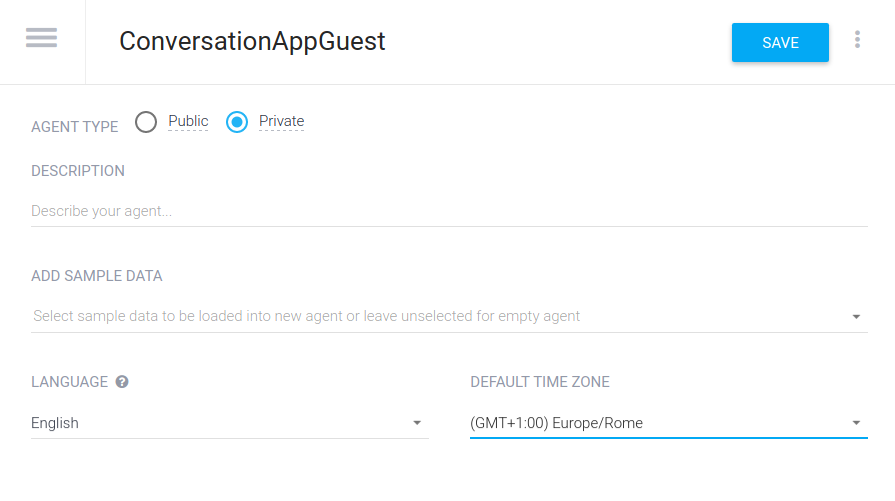
\includegraphics[width=0.7\textwidth,height=\textheight,keepaspectratio]{sezioni/images/saveagent.png}}
	\caption{save agent api.ai}\label{fig:saveAgent}
\end{figure}
Inserire nell'apposita schermata (figura \ref{fig:saveAgent}) i seguenti dati:
\begin{itemize}
	\item \textbf{Agent name}: ConversationAppGuest;
	\item \textbf{Agent type}: Private;
	\item \textbf{Language}: English;
	\item \textbf{Default time zone}: (GMT+1:00) Europe/Rome.
\end{itemize}
Cliccare poi "SAVE".\\
Successivamente, è necessario importare il primo agent applicando la seguente procedura:
\begin{itemize}
	\item selezionare l'agent appena creato nel menù a sinistra (figura \ref{fig:menuapi});
	\item cliccare il simbolo dell'ingranaggio, successivamente la voce "Export and Import" ed infine il pulsante "Import from zip" (figura \ref{fig:importAgent});
	\item l'agent da importare si trova nel repository scaricato (\ref{download}) in\\ \file{AtAVi/src/Back-end/VirtualAssistant/ApiAi/ConversationAppGuest}
\end{itemize}
\begin{figure}[h]
	\centering{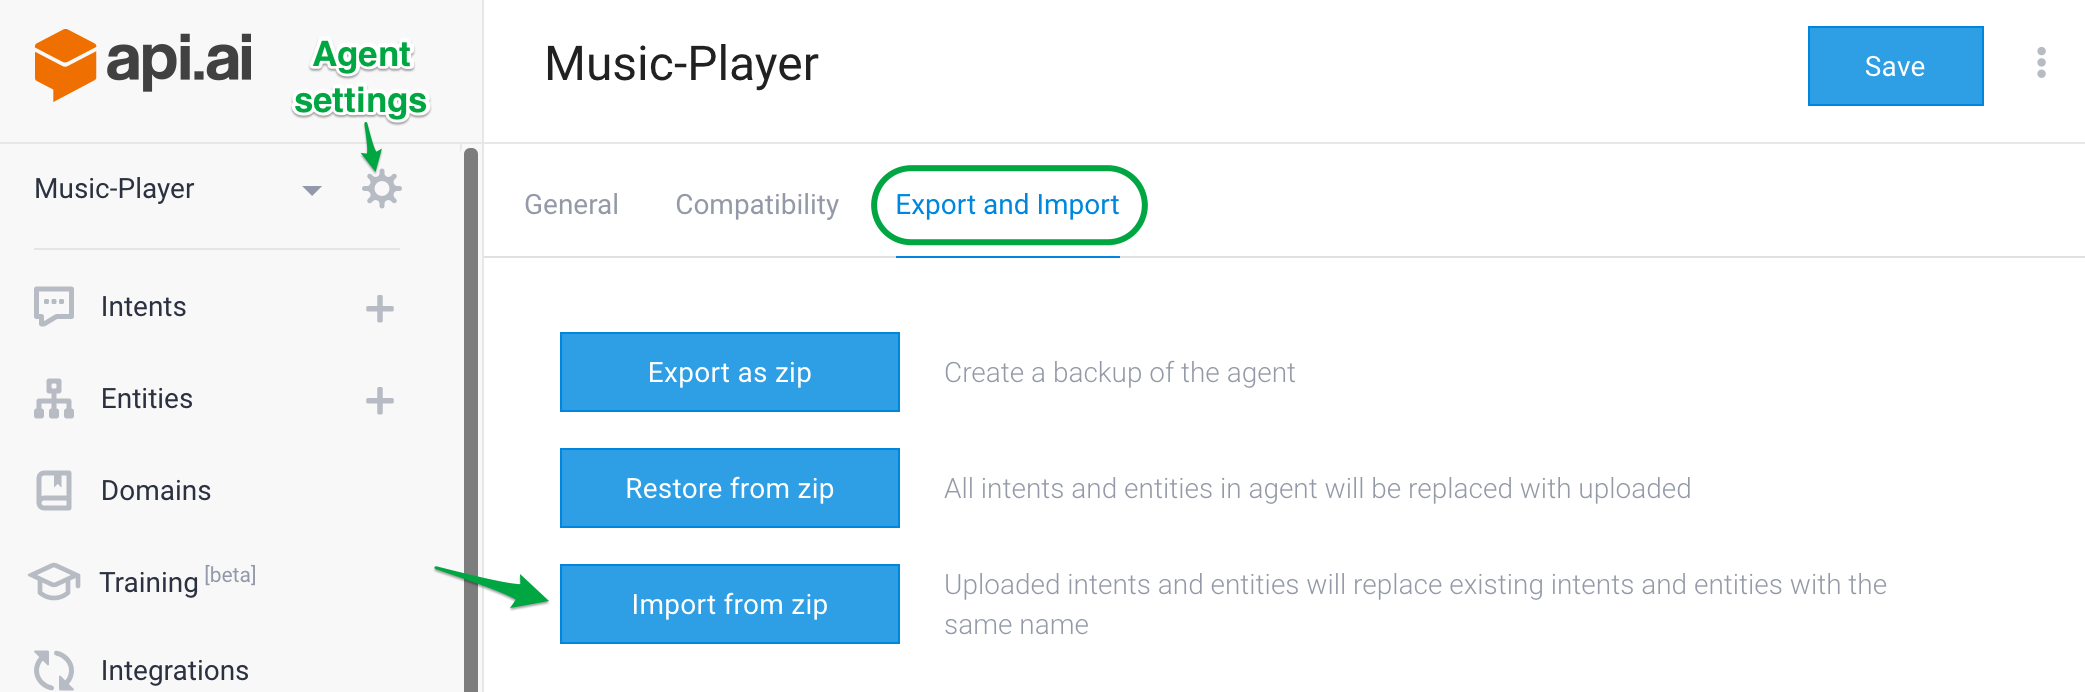
\includegraphics[width=1\textwidth,height=\textheight,keepaspectratio]{sezioni/images/importagent.png}}
	\caption{import agent api.ai}\label{fig:importAgent}
\end{figure}

Creare un secondo agent, chiamato "ConversationAppAdmin" e con percorso\\ \file{AtAVi/src/Back-end/VirtualAssistant/ApiAi/ConversationAppAdmin}, seguendo le istruzioni appena esposte.

??? SETTARE LE CREDENZIALI NEL SOFTWARE ???


\subsection{Deploy}
Una volta completate le procedure descritte in \ref{configurazione} e \ref{download}, si può procedere al deploy dei microservizi, dell'API Gateway, del Topic SNS e delle Lambda Function create.\\
Per farlo, è sufficiente dare il comando \file{sls deploy} (oppure \file{serverless deploy}) con il terminale aperto nelle seguenti cartelle:
\begin{itemize}
	\item \file{AtAVi/src/Back-end/APIGateway};
	\item \file{AtAVi/src/Back-end/VirtualAssistant};
	\item \file{AtAVi/src/Back-end/Notifications};
	\item \file{AtAVi/src/Back-end/Rules};
	\item \file{AtAVi/src/Back-end/Users};
	\item \file{AtAVi/src/Back-end/Events};
\end{itemize}

??? QUI DOVREMMO SCRIVERE COSE SU TIPO ADMIN DI DEFAULT O INIZIALIZZAZIONI NEI DB ???